\chapter{Stand der Forschung}
\section{Gold Standard}
% Was definiert einen guten Gold Standard?
Öffentliche Datensätze, welche Daten in Textform beinhalten, sind in verschiedenen Kategorien verfügbar\footnote{\url{https://medium.com/@dataturks/rare-text-classification-open-datasets-9d340c8c508e}}.
Auch Datensätze, die Informationen über Menüs beinhalten, sind bereits öffentlich verfügbar\footnote{\url{https://data.world/data-society/discover-the-menu}}.
Deutsche Textdatensätze sind bereits weniger verbreitet wie solche in englischer Sprache, jedoch sind ebenfalls welche frei verfügbar\footnote{\url{http://wortschatz.uni-leipzig.de/en/download/}}.
Einen Datensatz, welcher auf der deutschen Sprache basiert und Informationen über Menüseiten beinhaltet, konnte jedoch nicht gefunden werden, daher ist die Erarbeitung eines solchen Datensatzes Teil dieser Arbeit.
\section{Klassifikation}
Eine Methode, um Text in verschiedene Kategorien zu klassifizieren, ist das Erstellen von Regeln.
Mit einem ausgefeilten Regelsatz kann dies bei einer geringen Anzahl verschiedener Kategorien gut funktionieren \cite[p.125]{jackson2007natural}.
Das Erstellen eines solchen Regelsatzes ist zeitaufwendig und muss mit einem repräsentativen Datensatz überprüft werden \cite[p.125]{jackson2007natural}.
Somit ist es ein iterativer Prozess und der Ersteller muss sich im Themengebiet gut auskennen \cite[p.125]{jackson2007natural}.
Solche Regelsätze bestehen aus \glqq Wenn-Dann\grqq-Bedingungen, welche mit logischen \glqq UND\grqq{} bzw. \glqq ODER\grqq{} Operatoren verknüpft sind in Kombination mit regulären Ausdrücken \cite[p.126]{jackson2007natural}.
Mit solchen Regelsätzen könnten zwar hohe Scores erreicht werden, ein grosses Problem des Erstellens solcher Regelsätze ist der Zeitaufwand, denn dieser steigt linear mit der Komplexität \cite[p.127]{jackson2007natural}.
Aus diesem Grund besteht ein hoher Bedarf, Daten mittels statistischer Methoden automatisiert zu klassifizieren, ohne dass ein Mensch zuerst neue Regelsätze implementieren muss \cite[p.127]{jackson2007natural}.\\
An diesem Punkt kommen Machine-Learning-Algorithmen zum Zug.
Diese analysieren einen Datensatz, bei dem die Proben bereits eine Zuteilung zur jeweiligen Kategorie hinterlegt haben, und klassifiziert künftige Daten anhand dieser Analyse \cite[p.127]{jackson2007natural}. 
\section{No-Free-Lunch Theorem}\label{sec:nofreelunch}
Ein Theorem vom bekannten Informatiker David H. Wolpert, welches sinngemäss die Aussage trifft, dass kein Klassifizierer existiert, welcher für eine Vielzahl von Klassifikationsproblemen geeignet wäre\cite[p.]{Wolpert1996TheLO}.

\section{Klassifikationsalgorithmen}	% stand der forschung evt. classification von web pages?
\begin{itemize}
	\item Naive Bayes Modelle
	\begin{itemize}
		\item Bernoulli-Naive-Bayes
		\item Complement-Naive-Bayes
		\item Multinomial-Naive-Bayes
		\item Gaussian-Naive-Bayes
	\end{itemize}
	\item Nearest Neighbor Modelle
	\begin{itemize}
		\item KNeighborClassifier
		\item Nearest Centroid
	\end{itemize}
	\item Support Vector Machines Modelle
	\begin{itemize}
		\item LinearSVC (Support Vector Classification)
	\end{itemize}
\end{itemize}
\subsection{Lineare Modell}
Lineare Modelle sind in der Annahme, dass ein linearer Zusammenhang zwischen Eingangsvariablen und Ausgangsvariablen besteht.
Lineare Modelle versuchen Parameter zu einer linearen Gleichung zu finden, welche die Trainingsdatenpunkte optimal abdeckt.
Das optimale Abdecken wird mit einer Loss-Funktion ermittelt.
Die Loss-Funktion berechnet den Unterschied zwischen vorhergesagtem Wert zu tatsächlichem Wert des Trainingsdatenpunktes.
Lineare Modelle verwenden Optimierungsverfahren, welche iterativ Parameter verändern, um die Werte der Loss-Funktion zu minimieren und somit die bestmögliche Parameterzusammensetzung zu ermitteln.
\subsubsection{Ridge Classifier}
Ridge Classifier ist ein linearer Klassifizierer, welcher als Loss-Funktion die \glqq Least Square\grqq{} Funktion (eine Minimierung der quadrierten Abweichungen) und als Regularisierung die L2-Norm verwendet. Die L2-Norm wird pythagoreisch aus den Vektorwerten berechnet\footnote{\url{https://machinelearningmastery.com/vector-norms-machine-learning/} abgerufen am: 13.07.2019}.
Die Kombination aus oben erwähnter Loss-Funktion und der L2-Norm wird auch \glqq Ridge Regression\grqq{} genannt, von welcher der Klassifizierer auch seine Bezeichnung erhielt\footnote{\url{https://scikit-learn.org/stable/modules/generated/sklearn.linear_model.Ridge.html} abgerufen am: 13.07.2019}\cite{scikit-learn}.
\subsubsection{Passive Agressive Classifier}
Der PassiveAggressive Classifier ist ein Klassifizierer für grosse Datenmengen.
Er ist verwandt mit dem Perceptron Algorithmus, da er keine Lernrate benötigt.
Der Klassifizierer funktioniert grob umschrieben so, dass wenn die Klassifizierung korrekt ist, er sich passiv verhält und seine internen Gewichte nicht anpasst.
Erst bei einer falschen Klassifizierung ändert seine interne Gewichte aggressiv, so dass die Fehlklassifizierung behoben wird\cite{crammer2006online}.
\subsubsection{SGDClassifier}
SGDClassifier gehört zur Familie der lineare Modelle\footnote{\url{https://scikit-learn.org/stable/modules/generated/sklearn.linear_model.SGDClassifier.html} abgerufen am: 14.05.2019}\cite{scikit-learn}.\\
Der \glqq Stochastic-Gradient-Descent-Classifier\grqq{} verwendet als Optimierungsvefahren das \glqq Stochastic Gradient Descent\grqq{} Verfahren\footnote{\url{https://scikit-learn.org/stable/modules/sgd.html} abgerufen am: 14.05.2019}.
Bei diesem Verfahren kommt der mathematische Gradient zum Einsatz.
Der Gradient zeigt bei Anpassungen der Parameter, immer in die Richtung mit der grössten Änderung des Outputs.
Der Output wäre in diesem Falle die Aufzeichnung des Loss-Funktion.\\
Der stochastische/probabilistische Anteil dieses Verfahrens bedeutet, dass bei der Optimierung jeweils nur ein Parameter zufällig ausgesucht und angepasst wird und seine Auswirkung anschliessend ermittelt wird.
Dies hat den Vorteil, dass die Trainingszeit optimiert werden kann und zugleich gute Werte erzielt werden können.\\
In der Abbildung \cref{fig:sgd} wird der Verlauf der Loss-Funktion aufgezeigt und wie der Gradient zu interpretieren ist.
\begin{figure}[H]	
	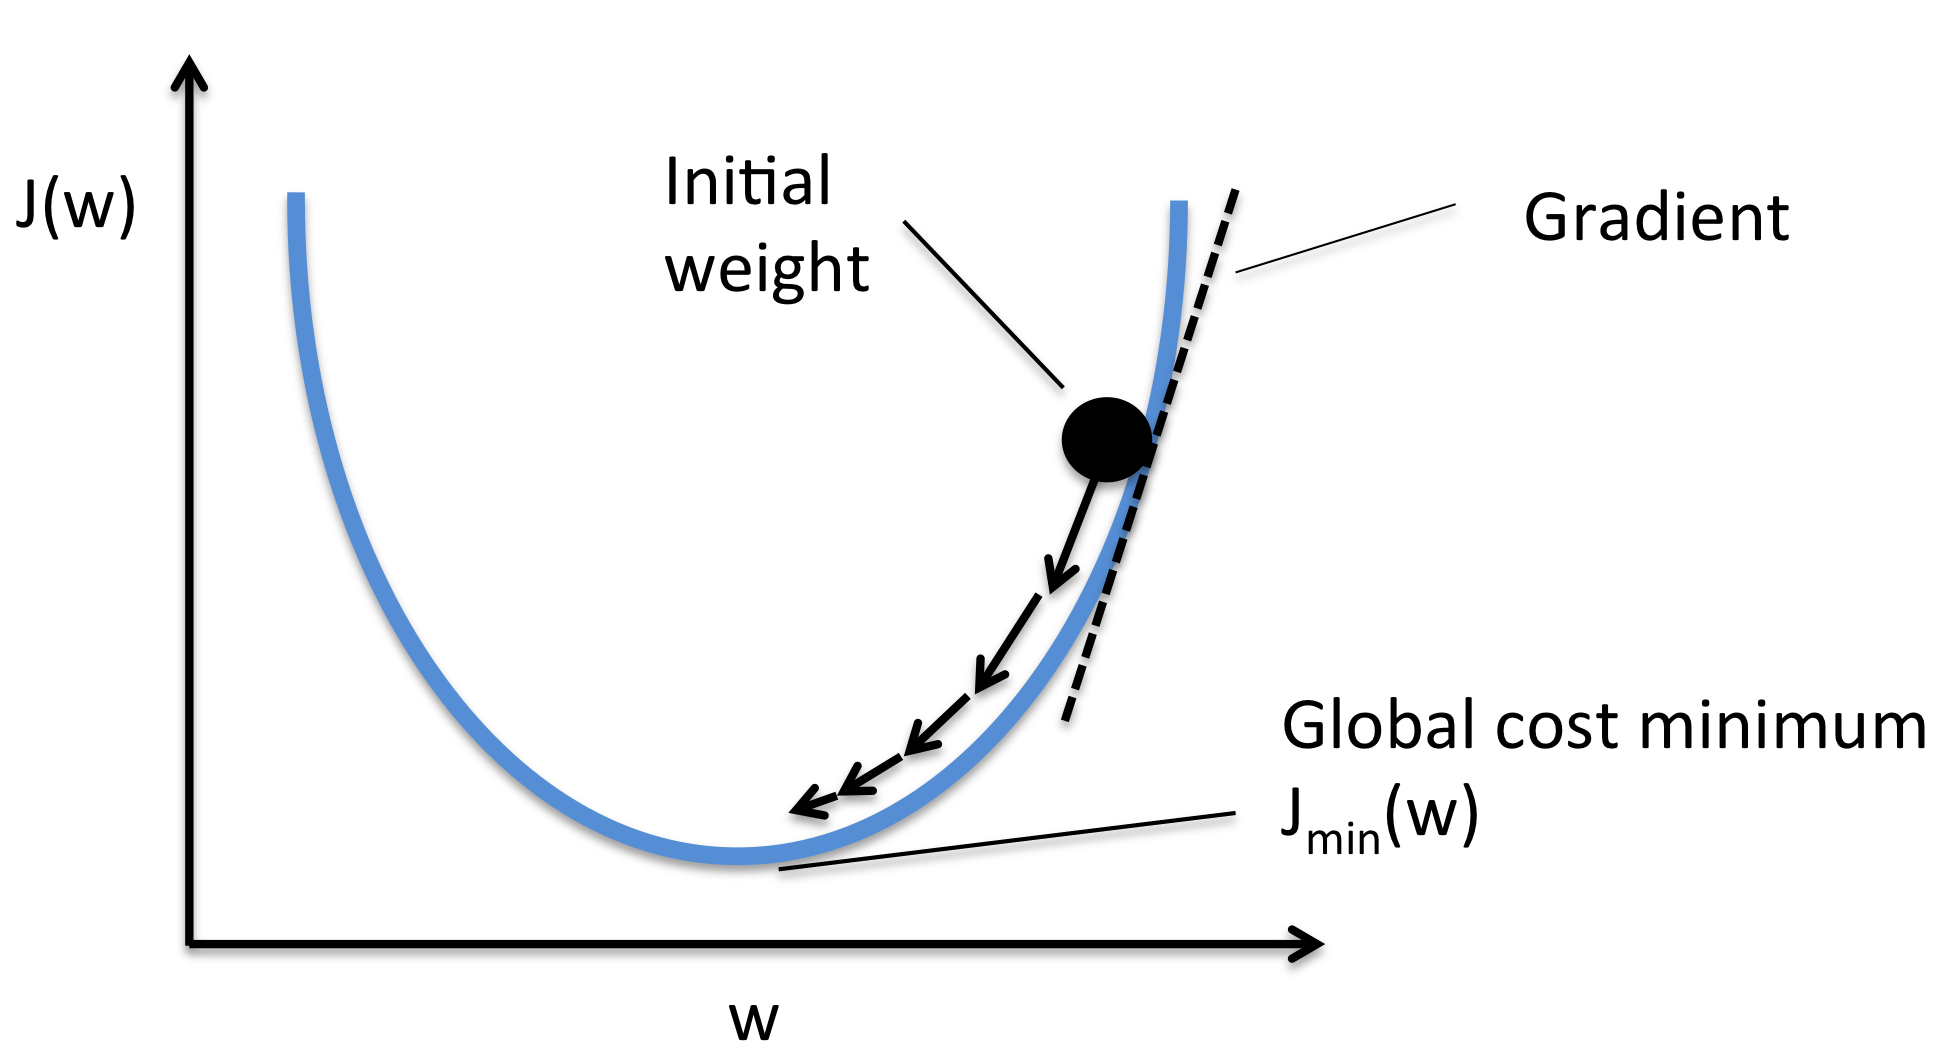
\includegraphics[width=1\columnwidth,keepaspectratio]{img/sgd.png}
	\caption{Visualisierung des Gradienten und der Loss-Funktion (J(w) = Loss; w = Parameteränderung)}
	\label{fig:sgd}
\end{figure}
\subsection{Perceptron}
Der Perceptron-Algorithmus basiert auf dem SGDClassifier\footnote{\url{https://scikit-learn.org/stable/modules/generated/sklearn.linear_model.Perceptron.html} abgerufen am: 14.05.2019}\cite{scikit-learn}.
Hinter der Perceptron-Implementierung steckt lediglich ein SGDClassifier mit spezieller Konfiguration.\\
Die Perceptron-Implementierung benutzt in der Konfiguration die Loss-Funktion \glqq perceptron\grqq{}, keine Strafe bei falscher Klassifizierung und eine konstante Lernrate.
\subsection{Naive Bayes}
\subsection{DecisionTree}\label{sec:trees}
Der DecisionTree-Algorithmus baut schrittweise eine Baumstruktur von Entscheidungszweige auf, um eine Klassifizierungsaufgabe zu meistern.
DecisionTrees versuchen eine komplexe Aufgabe in Teilprobleme zu zerlegen und diese mit einfachen Entscheidungen zu bewältigen.
DecisionTrees-Strukturen können verbessert werden, indem die Tiefe der Äste oder die Anzahl der Äste angepasst werden kann.
Bei stetiger Erhöhung der Tiefe oder der Anzahl der Äste, steigt auch die Zeitkomplexität der DecisionTrees\cite{safavian1991survey}.
\subsection{Ensemble-Learning}
Ensemble-Learning ist ein Zusammenschluss von mehreren unterschiedlichen Klassifizierern, welche mit einem Voting-Verfahren eine schlussendliche Klassifizierung durchführen.
Ensemble-Learning verfolgt die Annahme, dass mehrere Algorithmen im Plenum eine bessere Aussage abliefern können, als einen Algorithmus alleine\cite{freund1999short}.
\subsubsection{RandomForestClassifier}
RandomForest gehört ebenfalls zur Familie der Ensemble-Learner.\footnote{\url{https://scikit-learn.org/stable/modules/generated/sklearn.ensemble.RandomForestClassifier.html} abgerufen am: 14.05.2019}
RandomForest, wie der Name schon sagt, ist eine Zusammensetzung von einer Vielzahl von unterschiedlichen DecisionTrees \cref{sec:trees}.\\
RandomForest verwendet nun eine Vielzahl von DecisionTrees, die alle unterschiedliche Tiefen oder Anzahl Äste besitzen.
Dadurch können Entscheidungsausreisser aufgefangen und durch den Mehrheitsentscheid gedämpft werden\cite{liaw2002classification}.
\subsubsection{AdaBoostClassifier}
Bei vielen Ensemble-Verfahren werden alle Klassifizierer parallel trainiert und geben ihr Votum gleichzeitig ab.\\
Adaboost verwendet jedoch die Methode des \glqq Boosting\grqq{}, welche Ähnlichkeit mit der Theorie der genetischen Algorithmen hat\footnote{\url{https://scikit-learn.org/stable/modules/ensemble.html} abgerufen am: 14.05.2019}.
Bei Adaboost wird ein Algorithmus trainiert, validiert und als Ursprung verwendet. Alle zusätzlichen Algorithmen, welche das finale Voting durchführen, werden vom Ursprungsalgorithmus abgeleitet.
Es werden jedoch bei den Abkömmlingen die internen Parameter schrittweise verbessert und versucht die Fehler des \glqq Vater-Algorithmus\grqq{} zu vermeiden.
AdaBoost kann verbessert werden, indem die Anzahl von Vererbungsschritten angepasst wird\cite{freund1999short}.
\section{Hyperparametertuning}
Parameter, welche nicht selbstständig vom Machine-Learning Modell angepasst werden können, werden Hyperparameter genannt und sind meist Übergabeparameter in der Konstruktor-Methode.
Diese Hyperparameter definieren das Verhalten von den Modellen.
Die geeignetsten Hyperparameter können mit einer ausführlichen Suche gefunden werden, was als Hyperparametertuning bezeichnet wird\footnote{\url{https://scikit-learn.org/stable/modules/grid_search.html} abgerufen am: 14.05.2019}\cite{scikit-learn}.